\chapter{Spectral approximation properties of ReLU DNN}
Here we will talk about how to use ReLU DNN to approximate polynomials
and then achieve the ``spectral" accuracy for analytical functions.
The main results can be found in \cite{yarotsky2017error,
  wang2018exponential}. Some related works are
\cite{liang2016why,lu2017expressive}


First, we will introduce the following notation
\begin{itemize}
\item Colon notation for subscript: let $\{x_{m:n}\} = \{x_i:i =
  m,m+1,...,n\}$ and $\{x_{m_1:n_1,m_2:n_2}\}= \{x_{i,j}:i =
  m_1,...,n_1,j = m_2,...,n_2\}.$
\item Linear combination: denote $y\in \mathcal L(x_1,...,x_n)$ if
  there exist $\beta_i\in \mathbb{R},i=1,...,n,$ such that $y =
  \beta_0+\beta_1x_1+\cdots+\beta_n x_n$.
\item Linear combination with ReLU activation: denote $\tilde{y}\in
  \tilde{\mathcal L}(x_1,...,x_n)$ if there exists $y\in
  \mathcal{L}(x_1,...,x_n)$ and $\tilde{y} = \mbox{ReLU}(y) =
  \max(y,0).$
\end{itemize}
\begin{definition}
Given a function $f(x_1,...,x_d)$, if there exist variables $\{y_{1:L,1:M}\}$ such that 
\begin{equation}
y_{1,m}\in \tilde{\mathcal L}(x_{1:d}),\quad y_{l+1,m} \in \tilde{\mathcal L}(x_{1:d},y_{l,1:M}),\quad f\in\mathcal{L}(x_{1:d},y_{1:L,1:M}),
\end{equation}\label{def:netclass}
where $m=1,...,M,l=1,...,L-1$, then $f$ is said to be in the neural nets class $\mathcal{F}_{L,M}(\mathbb{R}^d)$, and $\{y_{1:L,1:M}\}$ is called a set of hidden variables of $f$. 
\end{definition}
\begin{properties}
A function $f\in \mathcal F_{L,M}(\mathbb R^d)$ can be represented by a ReLU network with depth $L+1$ and width $M+d+1$.
\end{properties}
\begin{proof}
Let $\{y_{1:L}\}$ be the hidden variables of $f$ that satisfies (\ref{def:netclass}), where
$$
f = \alpha_0 + \sum_{i=1}^d \alpha_1x_1+\sum_{l=1}^L\sum_{m=1}^M \beta_{l,m}y_{l,m}.
$$
Consider the following variables $\{h_{1:L,1:M}\}$:
$$
h_{l,1:M} = y_{l,1:M}, \quad h_{l,M+1:M+d} = x_{1:d}
$$
for $l = 1,...,L,$ and
$$
h_{1,M+d+1} = \alpha_0 + \sum_{i=1}^d\alpha_ix_i,\quad h_{l+1,M+d+1} =h_{l,M+d+1} + \sum_{m=1}^M\beta_{l,m}h_{l,m}
$$
for $l=1,...,L-1$. One can see that $h_{1,m}\in \tilde{\mathcal L}(x_{1:d}),h_{l+1,m}\in \tilde{L}(h_{l,1:M+d+1}),m = 1,...,M+d+1,l = 1,...,L-1,$ and $f\in \mathcal{L}(h_{L,1:M+d+1}),$ which is a representation of a standard neural net.
\end{proof}

\begin{properties}\label{prop:net class}
(Addition and composition of neural net class $\mathcal F_{L,M}$)
\begin{itemize}
\item[1]
$$
\mathcal F_{L_1,M} + \mathcal{F}_{L_2,M} \subseteq \mathcal{F}_{L_1+L_2,M},
$$
i.e. if $f_1\in \mathcal F_{L_1,M}(\mathbb{R}^d)$ and $f_2\in \mathcal{F}_{L_2,M}(\mathbb{R}^d),$ then $f_1+f_2\in\mathcal{F}_{L_1+L_2,M}(\mathbb{R}^d)$.
\item[2]
$$
\mathcal F_{L_2,M}\circ \mathcal F_{L_1,M+1} \subseteq \mathcal F_{L_1+L_2,M+1}.
$$ 
i.e. if $f_1(x_1,...,x_d)\in \mathcal{F}_{L_1,M+1}(\mathbb{R}^d)$ and $f_2(y,x_1,...,x_d)\in \mathcal{F}_{L_2,M}(\mathbb{R}^{d+1}),$ then 
$$
f_2(f_1(x_1,...,x_d),x_1,...,x_d)\in \mathcal{F}_{L_1+L_2,M+1}(\mathbb{R}^d).
$$
\end{itemize}
\end{properties}

\begin{proof}
For the addition property, denote the hidden variables of $f_1$ and $f_2$ as $\{y_{1:L_1,1:M}^{(1)}\}$ and $\{y_{1:L_2,1:M}^{(2)}\}$. Let
$$
y_{1:L_1,1:M} = y_{1:L_1,1:M}^{(1)},\quad y_{L_1+1,L_1+L_2,1:M} = y_{1:L_2,1:M}^{(2)}. 
$$
By definition, $\{y_{1:L_1+L_2,1:M}\}$ is a set of hidden variables of $f_1+f_2$. Thus $f_1+f_2\in \mathcal F_{L_1+L_2,M}.$

For the composition property, let the hidden variables of $f_1$ and $f_1$ as $\{y_{1:L_1,1:M+1}^{(1)}\}$ and $\{y_{1:L_2,1:M}^{(2)}\}$. Let
$$
y_{1:L_1,1:M+1} = y_{1:L_1,1:M+1}^{(1)},\quad y_{L_1+1:L_1+L_2,1:M} = y_{1:L_2,1:M}^{(2)},
$$
$$
y_{L_1+1,M+1} =\cdots= y_{L_1+L_2} = f_1(x_1,...,x_d).
$$
One can see that $\{y_{1:L_1+L_2,1:M+1}\}$ is a set of hidden variables of $f_2(f_1(\bm x),\bm x)$, thus the composition property holds.
\end{proof}

\begin{definition}
Given a continuous function $\varphi(\bm{x}),\bm{x} \in [-1,1]^d$ and a continuous function class $\mathcal F([-1,1]^d),$ define the $L^\infty$ distance
$$
\mbox{dist} (\varphi,\mathcal F) = \inf_{f\in \mathcal F} \max_{\bm x \in [-1,1]^d} |\varphi(\bm{x}) - f(\bm{x})|.
$$
\end{definition}

\begin{properties}\label{prop:dis}
(Addition and composition properties for distance function)
\begin{itemize}
\item[1] Let $\varphi_1$ and $\varphi_2$ be continuous functions. Let $\mathcal F_{1}$ and $\mathcal F_2$ be two continuous function classes, then 
$$
\mbox{dist}(\alpha_{1}\varphi_1+\alpha_{2}\varphi_2,\mathcal{F}_1+\mathcal F_2)\le |\alpha_1|\mbox{dist}(\varphi_1,\mathcal F_1) + |\alpha_2|\mbox{dist}(\varphi_2,\mathcal F_2),
$$
where $\alpha_1$ and $\alpha_2$ are two real numbers.
\item[2] Assume that $\varphi_1(\bm x) = \varphi_1(x_1,...,x_d),\varphi_2(y,\bm x) = \varphi_2(y,x_1,...,x_d)$ satisfy $\varphi_1([-1,1]^d)\subseteq[-1,1]$. Let $\mathcal F_1([-1,1]^d),\mathcal F_2([-1,1]^{d+1})$ be two continuous function classes, then
$$
\mbox{dist}(\varphi_2(\varphi_1(\bm x),\bm x),\mathcal F_2\circ \mathcal F_1)\le L_{\varphi_2}\mbox{dist}(\varphi_1,\mathcal F_1) +\mbox{dist}(\varphi_2,\mathcal F_2)
$$
where $L_{\varphi_2}$ is the Lipschitz norm of $\varphi_2$ with respect to $y$.
\end{itemize}
\end{properties}
\begin{proof}
The additional property obviously holds. Now we prove the composition property. For any $f_1\in\mathcal F_1,f_2\in \mathcal F_2$, one has
\[
\begin{split}
|\varphi_2(\varphi_1(\bm x),\bm x) - f_2(f_1(\bm x),\bm x)|&\le |\varphi_2(\varphi_1(\bm x),\bm x) - \varphi_2(f_1(\bm x),\bm x)|+|\varphi_2(f_1(\bm x),\bm x)-f_2(f_1(\bm x),\bm x)|\\
& \le L_{\varphi_2} ||\varphi_1(\bm x) -f_1(\bm x)||_\infty +||\varphi_2(y,\bm x) - f_2(y,\bm x)||_\infty
\end{split}
\]
Take $f_1^* = \argmin_f ||\varphi_1(\bm x) - f(\bm x)||_\infty$ and $f_2^* = \argmin_f ||\varphi_2(y,\bm x) - f(y,\bm x)||_\infty$, then it is proved.
\end{proof}

\begin{lemma}\label{lem:xsquare}
The function $\varphi(x) = x^2,x\in [-1,1]$ can be approximated by deep neural nets with an exponential convergence rate:
$$
\mbox{dist}(x^2,\mathcal{F}_{L,2}([-1,1]))\le 2^{-2L}.
$$
\end{lemma}
\begin{proof}
Consider the function
$$
g(y) = \left\{\begin{split}
	&2y,&\quad 0\le y<1/2,\\
	&2(1-y),&\quad 1/2\le y\le 1,
	\end{split}\right.
$$
then 
\begin{equation}\label{func:g}
g(y) = 2y -4\mbox{ReLU}(y-1/2)
\end{equation}
in $[0,1]$. Define the hidden variables $\{y_{1:L,1:2}\}$ as follows:
\[
\begin{split}
 y_{1,1} = \mbox{ReLU}(x),&\quad y_{1,2}=\mbox{ReLU}(-x),\\
 y_{2,1} = \mbox{ReLU}(y_{1,1}+y_{1,2}),&\quad y_{2,2} = \mbox{ReLU}(y_{1,1}+y_{1,2}-1/2),\\
 y_{l+1,1} = \mbox{ReLU}(2y_{l,1}-4y_{l,2}),&\quad y_{l+1,2} = \mbox{ReLU}(2y_{l,1}-4y_{l,2}-1/2)\\
\end{split}
\]
for $l = 2,3,...,L-1$. Using induction, one can see that $|x| = y_{1,1}+y_{1,2}$ and 
\begin{equation}\label{func:glinduction}
g_l(|x|)=\underbrace{g\circ g\circ \cdots \circ g}_{l}(|x|) = 2y_{l+1,1}-4y_{l+1,2},\quad l=1,...,L-1,
\end{equation} 
for $x\in [-1,1]$. i.e.
\[
\begin{split}
g_l(|x|) &= g\left(g_{l-1}(|x|)\right)\\
         &= g(2y_{l,1}-4y_{l,2})\qquad (\mbox{Eq~(\ref{func:g})})\\
         &= 2(2y_{l,1}-4y_{l,2}) - 4\mbox{ReLU}(2y_{l,1}-4y_{l,2}-1/2)\qquad (g_{l-1}(|x|)\ge 0~\mbox{if}~x\in[0,1])\\
         &= 2\mbox{ReLU}(2y_{l,1}-4y_{l,2})- 4\mbox{ReLU}(2y_{l,1}-4y_{l,2}-1/2)\\
         & = 2y_{l+1,1} - 4y_{l+1,2}\\
\end{split}
\]
by induction, Eq (\ref{func:glinduction}) holds.
\begin{figure}[h]
	\centering
	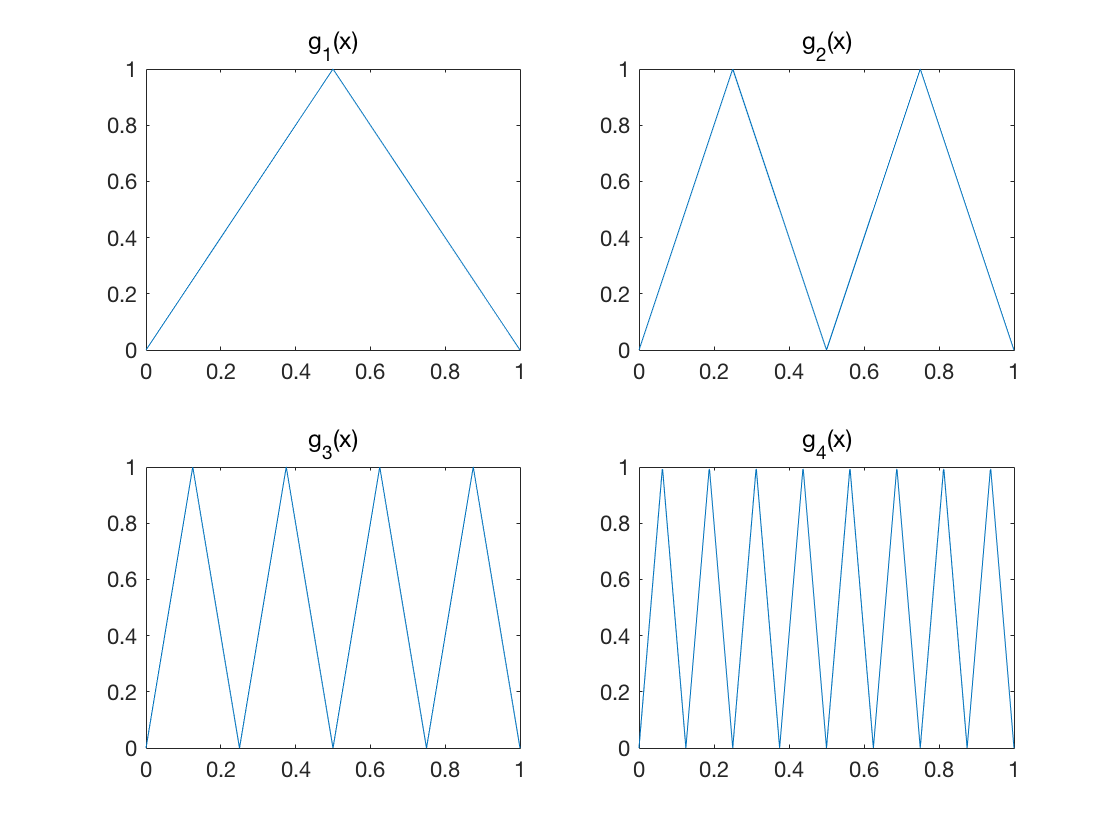
\includegraphics[width=0.8\textwidth]{dl_approx_analytic_gl}
	\caption{The figure of $g_l(x)$}
	\label{fig:gl}
\end{figure}

Let $f_m$ be the piecewise linear interpolation of $f$ with $2^m+1$ uniformly distributed breakpoints $\frac{k}{2^m},k = 0,...,2^m:$
$$
f_{m}(\frac{k}{2^m}) = (\frac{k}{2^m})^2,\quad k = 0,...,2^m.
$$
Note that refining the interpolation from $f_{m-1}$ to $f_m$ amounts to adjusting it by a function proportional to a sawtooth function:
$$
f_{m-1}(x) - f_m(x) = \frac{g_m(x)}{2^{2m}}.
$$
Hence 
$$
f_{L-1}(|x|) = |x| - \sum_{l=1}^{L-1}\frac{g_l(|x|)}{2^{2l}} .
$$
then $f_{L-1}\in \mathcal{F}_{L,2}$, and 
\[
\begin{split}
||x^2-f_{L-1}(x)||_{\infty} & = \max_{k} \max_{x\in [\frac{k}{2^{L-1}},\frac{k+1}{2^{L-1}}]} |x^2 - f_{L-1}(x)|\\
  & = \max_{k} |(\frac{1}{2}(\frac{k}{2^{L-1}}+\frac{k+1}{2^{L-1}}))^2 - f_{L-1}(\frac{1}{2}(\frac{k}{2^{L-1}}+\frac{k+1}{2^{L-1}}))|\\
  & = \max_k |(\frac{1}{2}(\frac{k}{2^{L-1}}+\frac{k+1}{2^{L-1}}))^2 - \frac{1}{2}((\frac{k}{2^{L-1}})^2+(\frac{k+1}{2^{L-1}})^2))|\\
  &=\frac{1}{4^L}.
\end{split}
\]
$|x^2-f_{L-1}(x)|\le 2^{-2L}$ for $x\in[-1,1].$
\end{proof}

\begin{lemma}\label{lem:xy}
For multiplication function $\varphi(x,y) = xy$, we have 
$$
\mbox{dist}(xy,\mathcal{F}_{3L,2}([-1,1]^2))\le 3\cdot 2^{-2L}.
$$
\begin{proof}
Notice that
$$
\varphi = xy = 2\left(\frac{x+y}{2} \right)^2-\frac{1}{2}x^2-\frac{1}{2}y^2.
$$
By properties \ref{prop:net class},\ref{prop:dis} and lemma \ref{lem:xsquare}, lemma \ref{lem:xy} is proved.
\end{proof}
\end{lemma}

\begin{lemma}
For a monomial $M_p(\bm x)$ of $d$ variables with degree $p$, we have
$$
\mbox{dist}(M_p,\mathcal F_{3(p-1)L,3})\le 3(p-1)\cdot 2^{-2L}.
$$
\end{lemma}

\begin{proof}
Let $M_p(\bm x)=x_{i_1}x_{i_2}\cdots x_{i_p},i_1,...,i_p\in\{1,...,d\}.$ Using induction, assume that the lemma holds for the degree-$p$ monomial $M_p$, consider a degree-$(p+1)$ monomial $M_{p+1}(\bm{x}) = M_p(\bm{x})\cdot x_{i_{p+1}}$. Let $\varphi(y,x) = yx,$ then $M_{p+1}(\bm x) = \varphi(M_p(\bm{x}),x_{i_{p+1}})$. We have
\[
\begin{split}
\mbox{dist}(M_{p+1},\mathcal{F}_{3pL,3})&\le \mbox{dist}(\varphi(M_p(\bm x),x_{i_{p+1}}),\mathcal F_{3L,2}\circ \mathcal F_{3(p-1)L,3})\\
& \le L_{\varphi}\mbox{dist}(M_p,\mathcal{F}_{3(p-1)L,3})+\mbox{dist}(\varphi,\mathcal F_{3L,2})\le 3p\cdot 2^{-2L}.
\end{split}
\]
Note that the Lipschitz norm $L_{\varphi}=1$ since $x_{i_{p+1}}\in [-1,1].$
\end{proof}

\begin{lemma}
For a degree-$p$ polynomial $P_p(\bm{x}) = \sum_{|\bm{k}|\le p}a_{\bm k}\bm x^{\bm k},\bm x\in [-1,1]^d,\bm k = (k_1,...,k_d)\in\mathbb{N}^d,$ we have 
\[
\mbox{dist}\left(P_p,\mathcal F_{\binom{p+d}{d}(p-1)L,3}\right)<3(p-1)\cdot 2^{-2L}\sum_{|\bm k|\le p}|a_{\bm k}|
\]
\end{lemma}\label{lem:poly}

\begin{proof}
This lemma can be proved by the properties \ref{prop:net class}, \ref{prop:dis} and lemma \ref{lem:poly}.
Note that the number of monomials of $d$ variables with degree less or equal to $p$ is $\binom{p+d}{d}$.
$$
k_1 + k_2 + \cdots + k_p \le p,
$$
Add a variables $k_{p+1}$, we have
$$
k_1 + k_2 + \cdots + k_p + k_{p+1} = p.
$$
the number of the non-negative solution is $\binom{p+d}{d}$.
\end{proof}

\begin{theorem}
Let $f$ be an analytic function over $(-1,1)^d$. Assume that the power series $f(\bm x) = \sum_{\bm k\in \mathbb N^d}a_{\bm k}\bm x^{\bm k}$ is absolutely convergent in $[-1,1]^d.$ Then for any $\delta>0,$ there exists a function $\hat f$ that can be represented by a deep ReLU network with depth $L$ and width $d+4$, such that
\[
|f(\bm x) - \hat f(\bm x)|<2\sum_{\bm k\in \mathbb N^d}|a_{\bm k}|\cdot \exp\left(-d\delta\left(e^{-1}L^{1/2d}-1\right)\right)
\]
for all $\bm x\in [-1+\delta,1-\delta]^d.$
\end{theorem}
\begin{proof}
Let $\epsilon = \exp(-d\delta(e^{-1}L^{1/2d}-1)),$ then $L = [e(\frac{1}{d\delta}\log\frac{1}{\epsilon}+1)]^{2d}$. Without loss of generality, assume $\sum_{\bm k}|a_{\bm k}|=1.$ We will show that there exists $\hat f\in \mathcal F_{L,3}$ such that $||f-\hat f||_{\infty}<2\epsilon.$
Denote 
$$
f(\bm x) = P_p(\bm x) + R(\bm x): = \sum_{|\bm k|\le p}a_{\bm k}\bm x^{\bm k} +  \sum_{|\bm k|> p}a_{\bm k}\bm x^{\bm k}.
$$
For $\bm x\in [-1+\delta,1-\delta]^d$, we have $|R(\bm x)|<(1-\delta)^p$, thus truncation to $p = \frac{1}{\delta}\log\frac{1}{\epsilon}$ with ensure $|R(\bm x)|<2\epsilon$. From lemma \ref{lem:poly}, we have dist$(P_p,\mathcal F_{L,3})<3(p-1)\cdot 2^{-2L'}$, where 
\[
\begin{split}
L' &= L\binom{p+d}{d}^{-1}(p-1)^{-1}\\
   &\ge L(\frac{(p+d)!}{p!d!})^{-1}p^{-1}\quad (d! \thicksim \sqrt{2\pi d}(d/e)^d)\\
   &\ge L(\frac{(p+d)^d}{(d/e)^d})^{-1}p^{-1}\\
   &= L[e(\frac{1}{d\delta}\log \frac{1}{\epsilon}+1)]^{-d}(\frac{1}{\delta}\log\frac{1}{\epsilon})^{-1}\\
   & = [e(\frac{1}{d\delta}\log \frac{1}{\epsilon}+1)]^{d}(\frac{1}{\delta}\log\frac{1}{\epsilon})^{-1}\\
   & \ge e^d (\frac{1}{\delta}\log\frac{1}{\epsilon}) \\
   &\gg\log\frac{1}{\delta}+ \log\frac{1}{\epsilon}
\end{split}
\]

for $d\ge 2$ and $\epsilon<<1$, then dist$(P_p,\mathcal F_{L,3})<<\epsilon$. Thus there exists $\hat f\in \mathcal F_{L,3}$ such that $||P_p - \hat f||_{\infty}<\epsilon$, and $||f-\hat f||_{\infty}\le ||R(x)||_\infty + ||P_p - \hat f||_\infty<3\epsilon$.
\end{proof}
for $d\ge 2$ and $\epsilon\ll 1$, then dist$(P_p,\mathcal F_{L,3})<3(p-1)\cdot 2^{-2L'} = 3(p-1)(\epsilon^2+\delta^2)\ll\epsilon$. Thus there exists $\hat f\in \mathcal F_{L,3}$ such that $||P_p - \hat f||_{\infty}<\epsilon$, and $||f-\hat f||_{\infty}\le ||f-P_p||_\infty + ||P_p - \hat f||_\infty<3\epsilon$.

